\chapter{Argumentation Framework} \label{ch:Argumentation Framework}
\section{Argumentation Framework}
Come i CSP l’argumentation è un altro metodo che offre l’intelligenza artificiale per rappresentare la conoscenza e risolvere i problemi. Quello che andremo a rappresentare sono delle situazioni/dialoghi che vogliamo studiare dal punto di vista logico.
\\Argumentation Framework. Un argumentation framework (AF) è una coppia (A,R) dove
\begin{itemize}
    \item A è un set di argomentazioni
    \item R $\subseteq$ A × A è una relazione rappresentante gli "attacchi" ("sconfitte")
\end{itemize}
\begin{center}
    $F(\{a,b,c,d,e\}, \{(a,b),(c,b),(c,d),(d,c),(d,e),(e,e)\})$
\end{center}
\begin{figure}[htp]
	\centering
    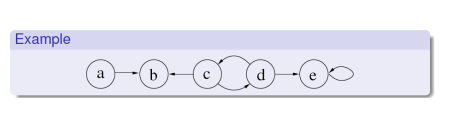
\includegraphics[width=12cm, keepaspectratio]{img/Cap6/arg1.png}
    \caption{Argumentation framework}
\end{figure}
Si ha un attacco quando si ha un’espressione logica (frase, dato...) che è in contraddizione con un’altra. Gli attacchi possono essere anche pesati, essi possono dipendere anche da chi ha detto quella frase.
\newpage
\begin{figure}[htp]
	\centering
    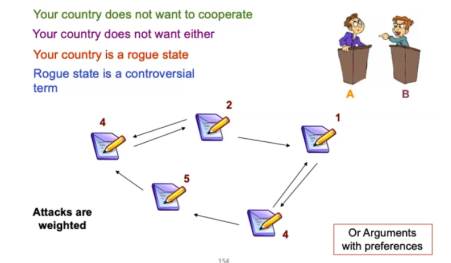
\includegraphics[width=12cm, keepaspectratio]{img/Cap6/arg2.png}
    \caption{Esempio di argumentation framework}
\end{figure}
Ci possono essere anche casi in cui è noto chi dice l’argomento e altri in cui non lo è. Per quest’ultima vogliamo selezionare gli argomenti che sono più validi rispetto agli altri, ad esempio in Figura 6.2 il 4 e il 2 sembrano buoni argomenti perchè attaccano gli altri e contrattaccano nel caso siano attaccati. Lo scopo è di definire dei criteri per trovare gli argomenti più forti, validi (che stanno "in piedi da soli"), in modo da selezione i conflitti che riescono a sopportare gli attacchi dall’esterno.
\begin{figure}[htp]
	\centering
    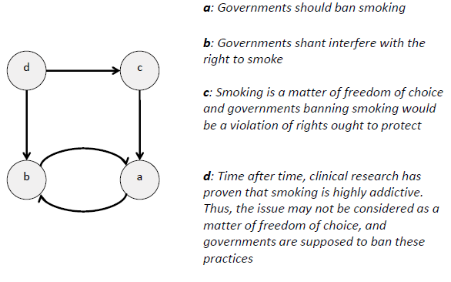
\includegraphics[width=12cm, keepaspectratio]{img/Cap6/arg3.png}
    \caption{Altro esempio di argumentation framework}
\end{figure}
Dobbiamo trovare gli argomenti che "stanno bene insieme", la prima nozione di questo tipo è un insieme di argomenti senza conflitti.
\section{Extension-Based Semantics}
Il task principale che viene svolto sugli argumentation framework è il computo della semantica, cioè si selezionano dei criteri con i quali si vanno a scegliere dei sottoinsiemi di argomenti che condividono una qualche proprietà particolare. La prima che vediamo è quella degli insiemi Conflict Free, cioè quegli insiemi che tra loro non hanno conflitti.
\subsection{Insiemi Conflict Free}
Dato un Augmentation Framework F = (A, R), l’insieme S $\subseteq$ A è conflict-free se, per ogni (a, b) $\in$ S, si ha che (a, b) $\notin$ R. (Per ogni coppia di elementi in S non è presente una relazione d’attacco tra questi elementi).
\begin{figure}[htp]
	\centering
    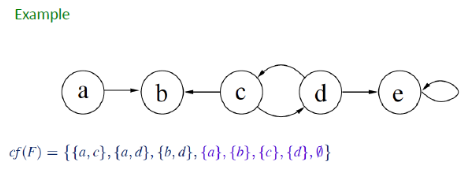
\includegraphics[width=12cm, keepaspectratio]{img/Cap6/cf.png}
    \caption{Esempio insieme conflict-free.}
\end{figure}
\\In questo caso andiamo a scegliere come coppie gli argomenti che non sono in conflitto (quindi che non si attaccano) fra di loro, ({a,c},{a,d} ma non {a,b}), e anche i singoli argomenti tranne e poichè esso si contraddice da solo visto che ha un cappio.
\begin{center}
    \textbf{Importante}
\end{center}
\textbf{Per il calcolo:} Inizio con inserire \textbf{l’insieme vuoto}, poi i \textbf{singoli} argomenti che non si auto-attaccano, poi \textbf{le coppie, terne, quadruple...}
\newpage
\subsection{Insiemi Ammisibili}
Dato un Augmentation Framework F = (A, R), l’insieme S $\subseteq$ A è ammissibile se:
\begin{itemize}
    \item S è \textbf{conflict free;}
    \item Ogni a $\in$ S è \textbf{difeso} da S (cioè ogni elemento che appartiene all’insieme è difeso dagli elementi dell’insieme stesso). Un elemento a $\in$ A è difeso da S se, per ogni b $\in$ A con (b, a) $\in$ R, esiste un c $\in$ S tale per cui (c, b) $\in$ R (a è difeso da S se per ogni b che attacca quell’elemento a esiste un altro elemento sempre dentro S che contrattacca l’attacco di b verso a).
\end{itemize}
\begin{figure}[htp]
	\centering
    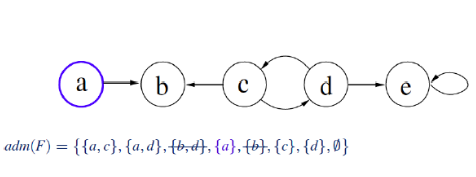
\includegraphics[width=12cm, keepaspectratio]{img/Cap6/ammissibile.png}
    \caption{Esempio insieme Ammisibile.}
\end{figure}
Non è necessario che sia lo stesso argomento a difendersi da altri attacchi, ad esempio in questo caso, supponendo che non ci sia a, b è attaccato da c ma se prendo d lui oltre che difendere se stesso da c (poichè attaccato) difende anche b. Guardando la definizione di difesa, un argomento a è difeso da un argomento b, (b, a) $\in$ R, nel momento in cui esiste un argomento c tale che c attacca b, (c, b) $\in$ R. Il sottoinsieme \{b,d\} non viene scelto poichè d è attaccato da c ma a si difende a sua volta contrattaccando, mentre b è attaccato sia da a che c, nel primo caso nessuno lo difende nel secondo d difende b perchè attacca c.
\begin{itemize}
    \item insieme V vuoto è \textbf{ammissibile}? Si, nessuno lo attacca.
    \item insieme V vuoto è \textbf{Conflict Free}? Si.
\end{itemize}
\newpage
\subsection{Insiemi Completi (Tutti Difesi)}
Dato un Augmentation Framework F = (A, R), l’insieme S $\subseteq$ A è completo se:
\begin{itemize}
    \item S è ammissibile;
    \item Ogni a $\in$ A difeso da S è contenuto in S. Un elemento a $\in$ A è difeso da S se, per ogni b $\in$ A con (b, a) $\in$ R, esiste un c $\in$ S tale per cui (c, b) $\in$ R.
\end{itemize}
\begin{figure}[htp]
	\centering
    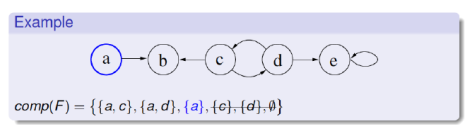
\includegraphics[width=12cm, keepaspectratio]{img/Cap6/completo.png}
    \caption{Esempio insieme Completo.}
\end{figure}
Quindi un insieme complete contiene tutti gli insiemi ammissibili e anche tutti gli argomenti che sono difesi.
\\Insieme V uoto è \textbf{Completo}? Va messo soltanto quando tutti gli argomenti sono attaccati e quindi quando \textbf{non} c’è un qualche argomento che è sempre difeso. 
\\Infatti sopra non va messo perchè a è sempre difeso. a è sempre difeso da tutti perchè non è attaccato da nessuno, quindi nel calcolo dei difensori va sempre messo dentro.
\begin{enumerate}
    \item \{a, c\} è \textbf{completo?} Si!
    \begin{itemize}
        \item a chi difende? attacca b quindi difenderebbe tutti quelli attaccati da b, ma b non attacca nessuno quindi a difende solo se stesso.
        \item c chi difende? tutti quelli attaccati da b quindi nessuno e tutti quelli attaccati da d quindi c.
    \end{itemize}
\textbf{L’insieme dei difensori è a, c, che sta dentro S=\{a, c\}, quindi è completo.}
\newpage
    \item \{a, d\} è \textbf{completo?}
    \begin{itemize}
        \item a chi difende? attacca b quindi difenderebbe tutti quelli attaccati da b, ma b non attacca nessuno quindi a difende solo se stesso.
        \item d chi difende? se stesso, perchè viene attaccato da c ma si difende da solo con un contrattacco.
    \end{itemize}
    L’insieme dei difensori è \{a, d\} che sta dentro S quindi anche questo è completo.
    \\\{a\} è \textbf{completo?} Può stare da solo perchè non viene attaccato da nessuno, quindi è \textbf{come se venisse difeso da tutti quanti}, e lui non difende nessuno, poichè b non attacca nessuno. 
    \\Quindi se un argomento non attaccato da nessuno ne attacca un altro che a sua volta non attacca nessuno allora quell’elemento è complete e può stare da solo.
    \\\{c\} è \textbf{completo?} Difensori: \{a, c\} che non è incluso in c quindi No.
    \\\{d\} è \textbf{completo?} Difensori: \{a, d\} quindi No. L’idea degli insiemi complete è che se un insieme difende qualcosa, quel qualcosa ”deve essere messo dentro” e \textbf{deve rimanere ammissibile.}
    
    \vspace{0.8cm}
    
    La differenza quindi è che nell’insieme ammissibile vuol dire che mi difendo, complete vuol dire che dentro ci sono tutti quelli difesi.
\end{enumerate}
\newpage
\subsection{Estenzioni Grounded (minimale)}
F = (A, R), l’insieme S $\subseteq$ A è grounded se:
\begin{itemize}
    \item S è \textbf{completo};
    \item Per ogni sotto insieme T $\subseteq$ A completo in F si ha che T $\subsetneq$ S
\end{itemize}
Quindi un insieme completo è grounded se è il \textbf{più piccolo dei complete}, ovvero se \textbf{non} esiste un sottoinsieme T complete che è più piccolo di lui. Si calcola tramite \textbf{l’intersezione} delle complete.
\textbf{N.B} L’insieme grounded è sempre \textbf{UNICO}, cioè composto da un solo elemento.
\begin{figure}[htp]
	\centering
    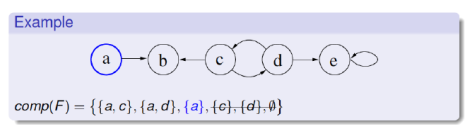
\includegraphics[width=12cm, keepaspectratio]{img/Cap6/completo.png}
    \caption{Esempio Grounded}
\end{figure}
\\a, c è \textbf{grounded}? i suoi sottoinsiemi singoli sono a e c, questi sono completi?
\\no, perchè a lo è ma non c quindi non è grounded.
\\a, d è \textbf{grounded}? i suoi sottoinsiemi singoli sono a e d, questi sono completi?
\\no, perchè a lo è ma non d quindi non è grounded.
\\a è \textbf{grounded}? Si, i suoi sottoinsiemi singoli sono a ed è completo.

\vspace{0.8cm}

\textbf{N.B} L’insieme grounded è dato anche dall’intersezione di tutti gli insiemi completi, infatti sopra se intersechiamo quei 3 insiemi completi l’unica cosa che viene fuori era a che infatti è l’unico insieme grounded.
\newpage
\subsection{Estenzioni Preferred (massimale)}
Dato un Augmentation Framework F = (A, R), l’insieme S $\subseteq$ A è preferred se:
\begin{itemize}
    \item S è ammissibile;
    \item Per ogni sotto insieme T $\subseteq$ A ammissibile in F , si ha che S $\subsetneq$ T (cioè se nessuno degli ammissibili S è più grande di T).
\end{itemize}
\begin{figure}[htp]
	\centering
    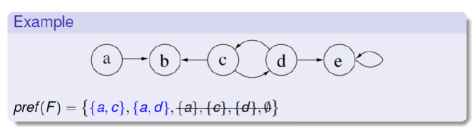
\includegraphics[width=12cm, keepaspectratio]{img/Cap6/prefered.png}
    \caption{Esempio Preferred}
\end{figure}
Si ottiene per inclusione insiemistica, \textbf{Le più grandi delle admissible}. (a) da solo è contenuto in (a,c) che è più grande quindi sicuramente non sarà preferred, stessa cosa per (d). (c) stessa cosa per (a,c).
\\Al contrario di grounded dove si andava a scegliere l’insieme con l’elemento in
comune con gli altri insieme, in questo caso si va a scegliere tra gli insiemi ammissibili
quelli che sono più grandi. Da notare che si sceglie tra gli insiemi ammissibili ma si
può dimostrare che si può scegliere da quelli complete.
\newpage
\subsection{Estenzioni Stable}
Dato un AF, F=(A,R). Un insieme S $\subseteq$ A è stabile in F, se
\begin{itemize}
    \item S è \textbf{conflict-free} in F
    \item per ogni a $\in$ A / S, esiste una b $\in$ S, tale che (b, a) $\in$ R.
\end{itemize}
\begin{figure}[htp]
	\centering
    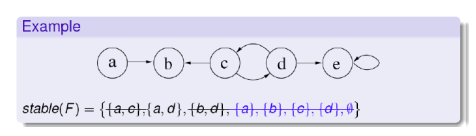
\includegraphics[width=12cm, keepaspectratio]{img/Cap6/stable.png}
    \caption{Esempio Stable}
\end{figure}
Per ogni elemento fuori da S esiste un elemento di S che lo attacca. Questo significa che gli insiemi stable sono gli insiemi conflict-free che attaccano tutti gli altri, ovvero che tutti gli elementi che stanno fuori dall’insieme esaminato sono attaccati.

\vspace{0.8cm}

In questo caso si sceglie l’insieme i quali elementi attaccano tutti gli elementi fuori dall’insieme conflict-free, ad esempio \{a,c\} non si prende perchè a attacca b e c attacca d e b ma nessuno dei due attacca e. Mentre nell’insieme \{a,d\} a attacca b e d attacca sia c che e. Esiste anche una semantica semi-stabile la quale nel caso cui esista un insieme stabile allora essa coincide con quest’ultimo ma quando non c’è la stabile allora sceglie tra gli insieme preffered quelli che ne attaccano di più tra gli insiemi fuori a quest’ultimo. L’obiettivo della semantica stabile è di avere cardinalità più grande possibile e di attaccare tutti gli insiemi fuori.

\vspace{0.5cm}

a, c \textbf{non è stabile} perchè è si ammissibile (b che sta fuori è attaccato e ok), d sta fuori ed è attaccato, ma e non lo attacca ne a ne c quindi questo insieme non può essere stabile.
\\a, d \textbf{è stabile} perchè a attacca b e d attacca c, e quindi tutti gli elementi fuori dall’insieme sono attaccati.
\\La semantica stabile è la più forte di tutte le estenzioni, perchè sono le posizioni più forti in un dialogo, sono la scelta migliore quando utilizzo AF come decision making. Il problema delle estenzioni stabili è che non sempre esistono.
\section{Soft Argumentation Framework}
Un Soft Argumentation Framework è una quadrupla:
\begin{center}
    $(A_{rgs} , R, W, S)$
\end{center}
dove:
\begin{itemize}
    \item $A_{rgs}$ è un insieme di Argomenti.
    \item R è una relazione di attacco sugli argomenti in $A_{rgs}$.
    \item W : $A_{rgs}$ x $A_{rgs}$ $\rightarrow$ S è una funzione binaria che rappresenta il peso associato ad ogni arco.
    \item S è un semiring $< A, +, x, bottom, top >$ Dati a, b $\in$ Args , $\forall$(a, b) $\in$ R, W (a, b) = s significa che a attacca b con un peso di s $\in$ S.
\end{itemize}
 Esempio:
\begin{figure}[htp]
	\centering
    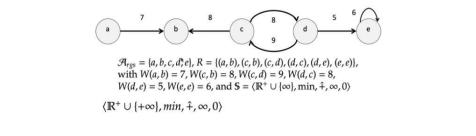
\includegraphics[width=13cm, keepaspectratio]{img/Cap6/SoftA.png}
\end{figure}
\\\textbf{Cambia la nozione di attacco:} Prima l’attacco era una funzione booleana (a attacca b). Adesso invece quando a attacca b gli viene associato un valore (comunque appartenente al semiring).
\\\textbf{Cambia la nozione di difesa:} Nell’esempio sopra, nel caso in cui fossimo negli AF tradizionali C si difenderebbe dall’attacco di D (perchè ricordiamo era una funzione booleana). In questo caso però, essendo che d attacca c con 9 e c risponde con 8, c non potrà difendersi dall’attacco, poichè la difesa non è sufficiente a contrastare quest’ultimo. Questa nozione dipende strettamente dal semiring utilizzato, poichè per ogni semiring (i cui tipi sono gli stessi introdotti precedentemente) si avranno relazioni diverse.
\subsection{w-difesa (Dw)}
Dato un Soft Argumentation Framework $(A_{rgs} , R, W, S)$, un sottoinsieme di argomenti B $\subseteq$ Args w-difende un argomento b $\in$ Args se e soltanto se, dato a $\in$ Args tale per cui R(a, b), allora:
\begin{center}
    $W (a, B \cup \{b\}) >=_s s W (B, a)$
\end{center}
L’insieme B w-difende l’elemento b se e soltanto se difende b da tutti gli attacchi che arrivano a b cioè da tutti gli R(a, b).
\\$>=_S$ è da intendere come elemento migliore o peggiore all’interno del semiring.
\\In altre parole, devo verificare che il peso degli attacchi che ricevo sia inferiore al peso degli attacchi che invio.
\begin{itemize}
    \item Con W (a, B $\cup$ \{b\}) si intende il costo degli attacchi che vanno da a all’insieme B $\cup$ \{b\} (cioè tutti gli attacchi che apporta quell’elemento a all’insieme B "dall’esterno verso l’interno") sommati con l’operatore di combinazione del semiring. Per sapere quindi quanto vale l’attacco di a verso l’insieme B $\cup$ \{b\} nel caso di Semiring Weighted ad esempio devo fare la somma di tutti gli attacchi (proprio perchè l’operatore di combinazione è la somma).
    \item W (B, a) sarebbe "con quanto l’insieme B attacca a, cioè tutti gli attacchi dall’interno di B all’esterno". Anche questo dipende strettamente dal semiring, nel Weighted vanno tutti sommati.
\end{itemize}
\textbf{Esempio}
\begin{figure}[htp]
	\centering
    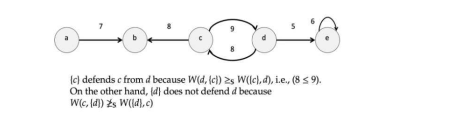
\includegraphics[width=12cm, keepaspectratio]{img/Cap6/srs.png}
\end{figure}
\\Per il calcolo degli insiemi ammissibili esistono vari metodi, che variano in base a regole imposte da autori di articoli scientifici.
\newpage
\subsection{Semantiche nei Weighted AF (W AAFs)}
\subsubsection{w-Conflict Free}
Dato un W F = $(A_{rgs} , R, W, S)$, un sottoinsieme di argomenti B $\subseteq$ Args è w-conflict free se e soltanto se W(B, B) = top (top del semiring). Questo significa che nessuno degli elementi dentro l’insieme attacca un altro elemento sempre dentro l’insieme. Dire che il peso è uguale al top del semiring (o al bottom) significa che quel peso non è presente, e quindi non è presente una relazione di attacco.
\subsubsection{w-Admissible}
Dato un W F = $(A_{rgs} , R, W, S)$, un insieme di argomenti B $\subseteq$ Args w-conflict-free è w-admissible se e soltanto se tutti gli argomenti di B sono w-difesi da B.
\section{Distinzione tra gli insiemi Admissible}
\subsection{Martinez e Simari (D1)}
L’obiettivo è capire se l’insieme B = \{b, c, d, e\} riesce a difendersi dall’attacco di a e poi dall’attacco di f , cioè se quell'insieme è ammissibile. Prendiamo in considerazione per tutti il semiring Weighted. Secondo Martinez e Simari non si aggregano ne le difese ne gli attacchi, quindi prendo il massimo degli attacchi ed il massimo delle difese.
\begin{figure}[htp]
	\centering
    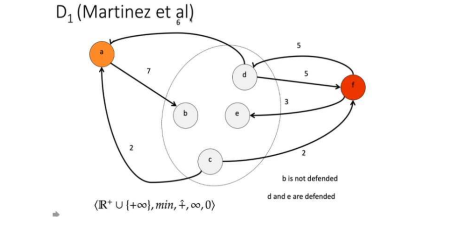
\includegraphics[width=12cm, keepaspectratio]{img/Cap6/martinez.png}
\end{figure}
\newpage
\textbf{Esempio:} Devo verificare che il \textbf{massimo} valore degli \textbf{attacchi} sia maggiore del \textbf{massimo} valore delle \textbf{difese}.
\\\textbf{Attacco} di a \textbf{verso} b:
\begin{itemize}
    \item Attaccanti (a): Max(7) = 7
    \item Difensori (d,c): Max(6,2) = 6
    \item Conclusione: 6 $<$ 7, b non è difeso e quindi non ammissibile
\end{itemize}
\textbf{Attacco} di f \textbf{verso} d, e:
\begin{itemize}
    \item  Attaccanti (f): Max(5,3) = 5
    \item Difensori (d,e): Max(5,2) = 5 (il 2 viene dall’attacco di c verso f)
    \item Conclusione: 5 = 5, (d), (e) sono difesi e quindi ammissibili.
\end{itemize}
La nozione formale di difesa in Simari-Martinez è: Dato W F = $(A_{rgs} , R, W, S)$, a, b, c $\in$ $A_{rgs}$ , B $\subseteq$ $A_{rgs}$ , allora b è difeso da B se per ogni R(a, b), esiste almeno uno c $\in$ B tale per cui W (a, b) $>=_s$ W (c, a).
\newpage
\subsection{Coste-Marquis (D2)}
Questo approccio aggrega solamente le \textbf{difese.}
\begin{figure}[htp]
	\centering
    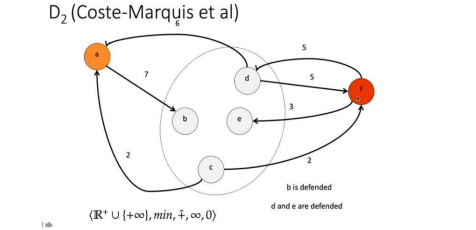
\includegraphics[width=12cm, keepaspectratio]{img/Cap6/marquis.png}
\end{figure}
\\\textbf{Attacco} di a \textbf{verso} b:
\begin{itemize}
    \item Attaccanti (a): Max(7) = 7
    \item Difensori (d,c): Difesa(6)+Difesa(2) = 6+2 = 8
    \item Conclusione: 8 $>$ 7, b è difeso e quindi ammissibile
\end{itemize}
\newpage
\subsection{Bistarelli e altri (Dw)}
Questo approccio aggrega \textbf{sia gli attacchi che le difese.}
\begin{figure}[htp]
	\centering
    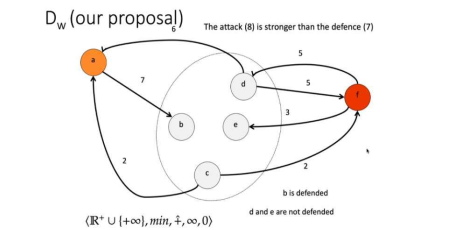
\includegraphics[width=12cm, keepaspectratio]{img/Cap6/bistarelli.png}
\end{figure}
\\\textbf{Attacco} di a \textbf{verso b:}
\begin{itemize}
    \item Attaccanti (a): Attacco(7) = 7
    \item Difensori (d,c): Difesa(6)+Difesa(2) = 6+2 = 8
    \item Conclusione: 8 $>$ 7, b è difeso e quindi ammissibile
\end{itemize}
\textbf{Attacco} di f \textbf{verso d, e:}
\begin{itemize}
    \item Attaccanti (f): Attacco(5)+Attacco(3) = 5+3 = 8
    \item Difensori (d,e): Difesa(5) + Difesa(2) = 7
    \item Conclusione: 8 $>$ 7, d, e \textbf{non} sono difesi e quindi non ammissibili.
\end{itemize}
\newpage
\section{Teoremi di implicazione tra le nozioni}
\textbf{N.B1 (da sapere):} La relazione di w-difesa implica la relazione di difesa:
\begin{center}
    B w-difende b $\rightarrow$ B difende b
\end{center}
\textbf{N.B2:} Nel semiring Classic (booleano) si ha che:
\begin{center}
    B w-difende a $\Leftarrow \Rightarrow$ B difende a
\end{center}
\begin{itemize}
    \item $D_W$ $\Rightarrow$ $D_2$ , Bista implica Costa-Marquis
    \item $D_1$ $\Rightarrow$ $D_2$ , Martinez implica Costa-Marquis
    \item Quindi se è ammissibile per Martinez e Bista allora è ammissibile anche per Costa-Marquiz
    \item Se S $=< [0, 1], max, min, 0, 1 > $ cioè semiring Fuzzy, allora D1 $\Leftarrow \Rightarrow$ D2
    \item Se $S =< [0, 1], max, min, 0, 1 >$ cioè semiring Fuzzy, allora Dw $\Leftarrow \Rightarrow$ D1
    \item Se $S =< [true, false], or, and, false, true >$ cioè semiring Classic, 
    \\allora $D_w \Leftarrow \Rightarrow D_0 \Leftarrow \Rightarrow D1 \Leftarrow \Rightarrow D_2$ (ma cosa è $D_0$ )??
\end{itemize}
\begin{figure}[htp]
	\centering
    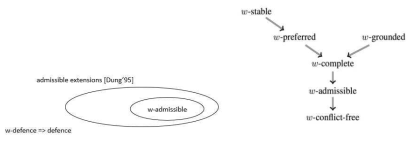
\includegraphics[width=12cm, keepaspectratio]{img/Cap6/teor.png}
\end{figure}
L’implicazione delle semantiche è la stessa sia nel caso classico che in quello pesato.
\newpage
\section{Orthogonal Relaxations}
\begin{figure}[htp]
	\centering
    
\includegraphics[width=12cm, keepaspectratio]{img/Cap6/ortogonal.png}
\end{figure}
In questo esempio notiamo che (d, c) non stanno bene insieme, perchè si attaccato 100. (b, c) sono abbastanza compatibili, perchè la relazione di attacco è presente ma con peso molto basso. Abbiamo poi che b non è ammissibile (non riesce a difendersi da c), c è ammissibile, d è ammissibile e nessuna
coppia di argomenti è ammissibile. Questo però non è una cosa positiva, perchè si vorrebbero cercare delle coalizioni superiori al singleton. Se però riuscissi ad accettare un po’ di conflitti interni potrei comunque creare una coalizione. Infatti notiamo che potremmo mettere insieme (b, c) dato che
la relazione di attacco è si presente ma con peso molto basso. Introduciamo quindi l’Alpha-hamma consistenza.
\newpage
\section{Alpha-Gamma consistenza}
Che cosa è l’\textbf{alpha-gamma consistenza?} Questa consistenza definisce il quantitativo di attacchi "interni" cioè alpha ed ”esterni” cioè gamma che si ammettono.
\begin{figure}[htp]
	\centering
    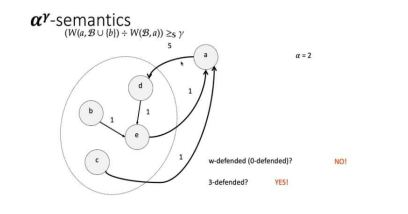
\includegraphics[width=12cm, keepaspectratio]{img/Cap6/cons.png}
\end{figure}
In questo esempio, l’insieme $B = \{b, c, d, e\}$ non è conflict-free (b e d attaccano e), però se volessimo misurare il valore di questo conflitto considerando il semiring Weighted (operazione somma), l’insieme è 2-conflict-free (infatti 2 elementi in questo insieme attaccano un altro elemento sempre appartenente all’insieme). Se quindi la soglia $\alpha$ fosse 2 riuscirei a sopportare l’attacco
tramite il rilassamento dei conflitti interni. Guardiamo l’ammissibilità dell’insieme: a attacca l’insieme B con 5 e B è difeso da 1 ed 1. In realtà l’argomento d andrebbe escluso dall’insieme
perchè porta un attacco con peso molto alto all’insieme stesso. Se però devo per forza costruire un organo di 4 elementi devo accettare sia i conflitti interni sia l’attacco verso d (potrei anche portare dentro a).
\subsubsection{Unità si sopportazione $\gamma$}
\textbf{N.B} secondo Bistarelli l’insieme B non è ammissibile, perchè l’attacco di 5 non è difeso dalla somma delle difese 1+1=2. Facendo il calcolo: (attacco-difesa) 5-2=3 si calcola l’unità di \textbf{sopportazione} $\gamma$ che in questo caso è 3.
\\Quindi:
\begin{itemize}
    \item $\alpha$ Peso del \textbf{conflitto interno} (in questo caso 2, dall’attacco di b pari ad 1 e d sempre 1 verso e)
    \item $\gamma$ Peso del \textbf{conflitto esterno} (in questo caso 3 (5 - 2))
\end{itemize}
L’insieme dell’esempio sopra è $2^3$ \textbf{admissible} perchè $\alpha$ = 2 e $\gamma$ = 3. Inoltre B è anche stabile, perchè tutti gli elementi esterni (in questo caso solo a) sono attaccati. Nel caso in cui portassimo d fuori si avrebbe un valore più basso di $\gamma$ ma B non sarebbe stato stabile, perchè nessuno attaccava d (a rimaneva comunque fuori).
\\
La semantica Alpha Gamma può essere descritta come:
\begin{center}
    $W (a, B \cup \{b\}) \div W (B, a)) >=_s \gamma$
\end{center}
dove:
\begin{itemize}
    \item $W (a, B \cup \{b\})$ : Il peso dell’attacco dall’esterno a verso l’interno B
    \item $\div$ : opposto della combinazione (x), abbiamo fatto esempi sempre con il Weighted, cioè la somma, quindi assumiamo sia la \textbf{sottrazione}
    \item W (B, a) Il peso dell’attacco dall’interno B verso l’esterno a
    \item Il risultato deve essere $>=_s$ $\gamma$ (migliore all’interno del semiring s).
\end{itemize}
L’insieme $B = \{b, c, d, e\}$ è anche $4^5$ \textbf{admissible}, e per dimostrare questo facciamo riferimento alle inclusioni.
\newpage
\subsection{Inclusioni in Alpha-Gamma consistenza}
\textbf{Teorema}: Dato un W F = $(A_{rgs }, R, W, S)$ con S = $(A, (+), (x), bottom, top)$ e $\alpha, \gamma \in$ A:
\begin{center}
    $\alpha^\gamma-stable \rightarrow \alpha^\gamma-prefered \rightarrow \alpha^\gamma-complete \rightarrow \alpha^\gamma-admissible \rightarrow \alpha-conflict-free$
\end{center}
\begin{figure}[htp]
	\centering
    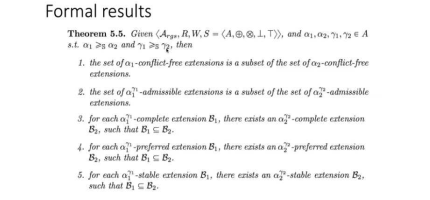
\includegraphics[width=12cm, keepaspectratio]{img/Cap6/alpha-gamma.png}
\end{figure}
\textbf{Le uniche cose spiegate dal prof nella figura sopra sono:}
\\Se un estenzione è $ \alpha_1$ ammissibile e $\alpha_1 >=_s \alpha_2$ allora quell’estenzione è anche $\alpha_2$ ammissibile. Stessa cosa per $\gamma$.
\\Questo significa che nell’esempio sopra che era $2^3$ admissible sarà anche $4^5$ ammissibile (ecco spiegata la domanda della sezione sopra).
\newpage
\section{Semantica w-Grounded}
Gli insiemi grounded sono gli insiemi complete più piccoli.
\\\textbf{Def di Grounded (Minimale) nel caso normale (Crisp AF):}
\begin{center}
    E $\in$ gr(F) if f E $\in$ co(F) e \textbf{non esiste} E' $\in$ co(f) tale per cui E' \textbf{non è contenuto} in E.
\end{center}
Un estenzione E è grounded se e solo se è una complete e nessun altra estenzione dentro le complete è più piccola di lei (quindi è la più piccola delle complete).
\begin{figure}[htp]
	\centering
    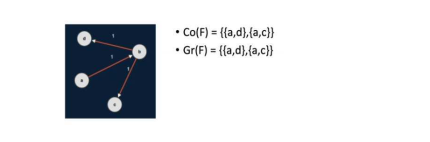
\includegraphics[width=12cm, keepaspectratio]{img/Cap6/w-grounded.png}
\end{figure}
\textbf{Calcolo delle complete se non ci fossero i pesi:} L’insieme complete era (a, d, c) perchè a difendeva sia d che c insieme. 
\\\textbf{Calcolo delle complete con pesi (usiamo Bistarelli):} Le complete in questo caso sono a perchè non viene attaccata da nessuno e più tutte quelle difese da a cioè d e c. \textbf{Non le difende tutte e due insieme} perchè il costo 1 non è sufficiente e difenderle tutte e due, deve per forza farlo uno alla volta (cosi ha detto il bista). Quindi le complete sono (a, d) e (a, c). Applicando la definizione di Grounded all’esempio otteniamo che l’insieme è sempre lo stesso delle complete, ma questo è un problema, perchè le grounded hanno la proprietà di essere \textbf{uniche}.
\\\textbf{Tutto quello sopra è per dimostrare che la definizione di Grounded con pesi negli AF va cambiata a}
\newpage
Un elemento E è Grounded se e soltanto se:
\begin{enumerate}
    \item \textbf{ É ammissibile} (prima si richiedeva che era complete);
    \item  É incluso nell’intersezione delle \textbf{complete};
    \item  Non esiste nessun elemento \textbf{ammissibile} più grande di E.
\end{enumerate}
\begin{figure}[htp]
	\centering
    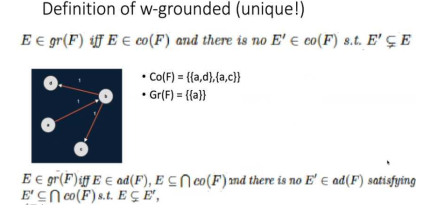
\includegraphics[width=12cm, keepaspectratio]{img/Cap6/w-gounded2.png}
\end{figure}
L’insieme degli ammissibili in questo caso era: (a), (a, c), (a, d) quindi l’intersezione viene a che è appunto l’unica grounded (e non è attaccata da nessuno).
\\Negli Weighted AF la definizione di Grounded va cambiata perchè altrimenti si perderebbe la proprietà di essere \textbf{uniche}.
\section{Argomento Scetticamente/Credulosamente accettato}
Trattiamo adesso un problema decisionale (quindi chiedere se un argomento è SI/NO), introducendo il significato di un argomento Credulosamente o \textbf{Skep/(Scet)ticamente }accettato su questo esempio
\newpage
\begin{figure}[htp]
	\centering
    
\includegraphics[width=12cm, keepaspectratio]{img/Cap6/scet.png}
\end{figure}
\begin{itemize}
    \item \textbf{Cred} (Almeno in un insieme): Ci domandiamo: esiste \textbf{almeno} una volta che l’argomento 2 compare in output? La domanda va posta in base a quello che calcoliamo, ad esempio, nel caso in cui calcolassimo le conflict-free e il 2 non compare tra le coppie che lo sono, la risposta sarà NO, mentre nel caso in cui comparisse in almeno una coppia (o anche da solo) la risposta sarebbe SI.
    \item \textbf{Skept} (In tutti gli insiemi): Se un elemento è \textbf{sempre} dentro un estenzione. In questo caso l’output sarà NO perchè non c’è un elemento che è comune a tutti gli insiemi. É possibile selezionare l’elemento, quindi magari per il valore 4 da NO, ma per il valore 3 da SI.
\end{itemize}
\begin{figure}[htp]
	\centering
    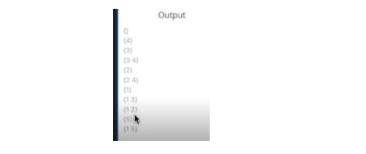
\includegraphics[width=12cm, keepaspectratio]{img/Cap6/skep.png}
\end{figure}
\newpage
\section{Tipologie di semantiche}
Esistono principalmente tre tipologie di semantiche basate sulla metodologia
con la quale vengono calcolate.
\begin{enumerate}
    \item \textbf{Estenzione:} Andiamo a guardare dei sottoinsieme di argomenti (tutte quelle viste precedentemente)
    \item \textbf{Labeling:} Il labeling è una funzione che assegna delle etichette (colori) ad ogni argomento in modo tale da distinguere gli argomenti accettati dai restanti.
    \item \textbf{Ranking:} Restituisce un ordimento sugli argomenti. Dice quindi "l’argomento a è migliore di b". Questo sistema è più raffinato.
\end{enumerate}
\section{Semantiche basate su Estenzione (ripetizione)}
\begin{itemize}
    \item \textbf{Conflict Free}: Argomenti che non si attaccano.
    \item \textbf{Ammissible}: Richiede la nozione di difesa, cioè un contrattacco che un argomento fa ad un altro argomento che è attaccato.
    \item \textbf{Complete}: Deve essere admissible, se un argomento è difeso questo è per forza dentro l’estenzione. Nell’esempio sopra a era l’unico argomento che era sempre difeso (non veniva attaccato da nessuno) quindi l’insieme complete sono tutti gli argomenti che hanno dentro a.
    \item \textbf{Prefered}: Si ottiene per inclusione insiemistica, cerco le admissible più grandi. tra \{a\},\{c\},\{d\},\{a, c\},\{a, d\} dato che voglio la più grande, la singola {a} non potrà essere prefered, perchè si trova dentro \{a, c\},\{a, d\} che sono più grandi.
    \item \textbf{Grounded}: Set più piccolo tra tutte le complete.
    \item \textbf{Stable}: Seleziono un insieme di argomenti che è conflict free e che attacca tutti gli altri
\end{itemize}
